\section{Durchführung der Aufgabe}

In diesem Kapitel beschreiben wir konkret, wie die Arbeit während meines Praxissemesters sich entwickelte. Die ersten zwei Wochen dienten als Einarbeitung und Einstieg. Nach dieser Phase bekam ich langsam und unter Betreuung mehr Verantwortung und mehr Freiheit, um die Arbeit durchzuführen. In der folgenden Tabellen wird der Ablauf systematisch und ohne Einzelheit beschrieben. In dem zweiten Teil dieses Kapitels geben wir eine ausführliche Beschreibung eines Projekts.

Jedes Projekt besitzt innerhalb von Wallsec einen festgelegten Aufbau. Dieser kann in den folgenden Punkten zusammengefasst werden:

\begin{enumerate} \label{Projektablauf}
    \item \textit{Kick-off Meeting} mit den Kunden, um grundsätzliche Informationen über die Anwendung zu bekommen
    \item Definition des Testumfangs, wie Anmeldedaten, Rolle der Nutzer, \glsplural{Tennant} und Einschränkungen
    \item Durchführung von Tests nach einer vorgegebenen Checklist
    \item Dokumentation der durchgeführten Testen, deren gefundene \glsplural{Schwachstelle} und Vorschläge zur Härtung der Anwendung
    \item Abschlussmeeting mit den Beauftragten, um die \glsplural{Schwachstelle} und deren Ausnutzung zu präsentieren und zu demonstrieren
\end{enumerate} 

\section{Wöchentliche Zusammenfassung meines Praxissemesters}

\begin{table}[H]
    \setstretch{1.0}
    \begin{tabularx}{\textwidth}{|c|X|}
    \toprule
    \multicolumn{2}{c}{\textbf{Auflistung der Aufgabe}} \\
    \midrule
    \multicolumn{1}{c}{\textbf{Woche}} & \multicolumn{1}{c}{\textbf{Aufgabeschreibung}} \\
    \hline
    1 - 2    & Einarbeitung:
                \begin{itemize}
                    \item Installation von einer virtuellen Maschine für die Testumgebungen
                    \item Einführung in der Arbeitsablauf der Firma
                    \item Einführung, Installation und Einstellungen von \gls{burp}
                    \item Einführung in einem laufenden Projekt, um über das Ablauf- und Dokumentationsverfahren zu lernen
                    \item Durchführung und Wiederholungen von einigen Tests, um mich an den gegebenen Tools zu gewöhnen
                    \item Teilnahmen an einer Abschlussmeeting des laufenden Projekts, um das Verfahren und den Ablauf des Kundenkontakt zu erkennen und später zu wiederholen
                \end{itemize} \\
        \hline

    3 - 4       &  Start, Durchführung und Abschluss eines neuen Pentesting-Projekts an einem Versicherungsanwendung mit dem obigen beschriebenen Schritte (\ref{Projektablauf})  \\ 
    
    \hline

    5 - 6       & Weiterarbeitung an der Installation, an der Einstellungen und an der Nutzung der Tools \gls{TheHive} und \gls{Cortex}. Bereitstellung von Skripts zum Herunterladen von statistische Daten der Anwendungen und zur Automatisierung deren Nutzung.  \\ 

    \hline

    7 - 8      &  Start, Durchführung und Abschluss eines neuen Pentesting-Projekts an einem Marketing-Webanwendung mit dem obigen beschriebenen Schritte (\ref{Projektablauf}) \\

    \hline

    9 - 10      &  Start, Durchführung und Abschluss eines neuen Pentesting-Projekts an Netzwerk-Umgebungen mit dem obigen beschriebenen Schritte (\ref{Projektablauf}). Die durchgeführten Tests konzentrieren sich auf die Sicherheit einer Netzwerk in einer Cloud-Umgebung. Für dieses Projekt spielen die Tools \gls{nmap} und \gls{scout} eine wichtige Rolle, da das Ziel war, Hosts, Dienste und dessen Einstellungen und \gls{Schwachstelle} zu erkennen \\

    \hline

    11  	    &  Start, Durchführung und Abschluss eines Pentesting bei einem umfangreichen Webanwendung mit verschiedenen \glsplural{Tennant} und Nutzungsrolle für die Verwaltung von Business-Processes. \\

    \hline

    11 - 12      &  Start, Durchführung und Abschluss eines Pentesting bei dessen Aufbau auf HTTP2 \textbf{GLOSSARhier} und \textbf{Graphisql}. Da diese Element mir ganz fremd waren, habe ich viel während der Testes davon gelernt, wie sie ausgenutzt werden können und deren Sicherheitslücke. \\


    \hline

    17 - 18      &  xxxxxx \\

    \hline

    19 - 20      &  xxxxxx \\


       \bottomrule
    \end{tabularx}
\end{table}

\section{Ausführliche Beschreibung eines Penetration Testing innerhalb des Praxissemesters}

Bevor der Durchführung jedes Tests ist Wallsec und ihre Mitarbeiter dazu verpflichtet, eine Vertraulichkeitserklärung zu unterschreiben. Keine Information weder über die Firma noch über die verwendeten Methode dürfen aus irgendwelcher Form veröffentlicht werden. Aus diesem Grund werden die hier demonstrierten Methode und Tests in der Test- und Lernumgebung \glsfirst{dvwa} gezeigt. In den realen Tests verwenden wir ähnliche Methode, manchmal mit mehr oder weniger Details, um die Sicherheit der Anwendungen zu überprüfen. 

Da dieses Bericht eingeschränkte Platz hat und das dieses Thema sehr umfangreich hier, demonstrieren wir in den nächsten zwei Unterkapitel einige Methode, die wir verwenden, um die Zielanwendung in ihrer Struktur zu kennen und auszunutzen.

\subsection{Sammlung von Informationen von dem Zielsystem}

Obwohl jede Webanwendungen ihre eigene Eingenschaften und Ziele haben, besitzen fast alle eine ähnliche Struktur und Aufbau. Beim jeden Test fangen wir damit an, diese gemeinsame Struktur zu erkennen, indem wir nach öffentlichen Informationen suchen. Viele kritische Informationen, wie Username, Passwörter, Versionen, Systemen verbundenen IP-Adressen, lassen sich nach einer Online-Suche finden. Auch mit eingebauten Tools eines Betriebssystems können wir auf solche Informationen zugreifen. Dieses Verfahren nennen wir Banner Grabbing. Das folgende Bild zeigt ein Beispiel von einer einfachen Durchführung von Banner Grabbing:

\begin{figure}[H]
    \centering
    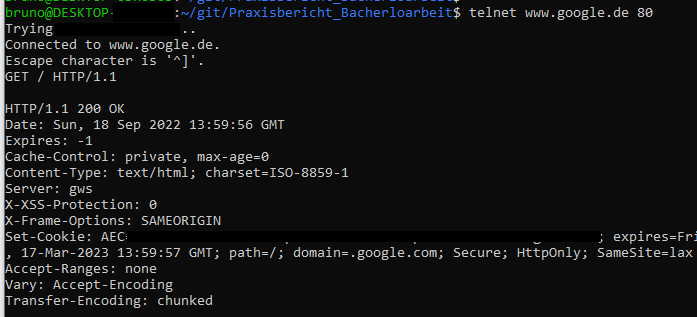
\includegraphics[width=0.5\textwidth]{/home/bruno/git/Praxisbericht_Bacherloarbeit/Praxissemester/assets/banner_grabbing.png}
    \caption{Banner Grabbing mithilfe von dem Tool telnet}
    \centering
\end{figure}

Eine Webanwendung ist eine Gruppierung von verschiedene Verzeichnisse. Jedes Verzeichnis soll den Nutzer eine Information oder Interaktion anbieten. Manche sind aber nicht für Nutzer gedacht und dient zur Verwaltung von Einstellungen. Da solche Verzeichnisse nicht direkt aufrubar sind  benutzen wir Testers andere Methode, um zu finden, was die Entwickler im Hintergrund beibehalten wollte. Es gibt verschiedene Tools, die mithilfe von sogenannten \textit{wordlists}, viele Anfrage an eine Anwendung schickt, um herauszufinden, was nicht direkt von dem Browser aufrufbar ist. Solche \textit{wordlists} sind Textdateien, die häufige verwendete Wörter beinhalten, die für Webanwendungen, für Nutzername oder für Passwörter verwendet werden. Da viele Webanwendungen ähnliche Strukturen haben, ist auch meistens erwartet, dass gewöhnliche Wörter auch zu finden sind. Das nächste Beispiel zeigt uns, dieses Entdeckungsverfahren auf unserem Ziel, \gls{dvwa} Tool. Hier benutzen wir das Tool \gls{dirb}, um herauszufinden, welche Verzeichnisse in dieser Anwendung existieren. In diesem Fall werden verschiedene Anfrage geschickt, jede mit einem verschiedenen Wort, um zu sehen, welche positive Antworten liefern. Das folgende Bild zeigt die Durchführung und das Ergebnis des Scanverfahren mithilfe des Tools \gls{dirb}:

\begin{figure}[H]
    \centering
    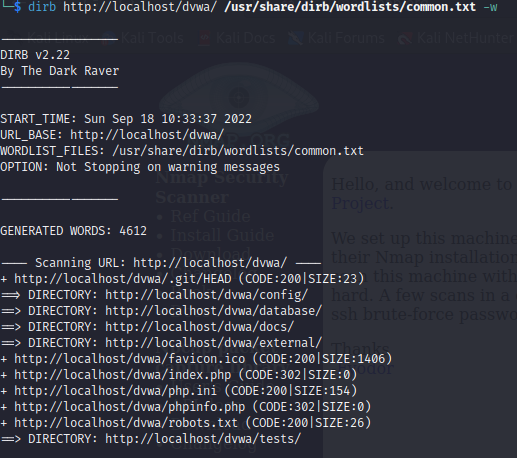
\includegraphics[width=0.5\textwidth]{/home/bruno/git/Praxisbericht_Bacherloarbeit/Praxissemester/assets/dirb.png}
    \caption{Brute force Scan für Verzeichnisentdeckung}
    \centering
\end{figure}

Der nächste Schritte wäre eine manuelle Beobachtung der entdeckten Material, um zu finden, ob irgendwelche sensitiven Information ausgelieferte wurde. Falls ja, wurden wir dann versuchen diese \gls{Schwachstelle}, zu erkennen und auszunutzen.

Ein Netzwerk-Scan ist auch eine häufige verwendete Methode, um Dienste innerhalb des testenden Objekts zu finden. Dieser Scan schickt an das Ziel verschiedene Anfrage, damit wir das Reaktion des Zielsystems beobachten können. Während bei dem ersten Scan wir uns auf der Webanwendung fokussierten, bearbeiten wir hier eine Ebene, die nicht für normale Nutzung gezielt ist. Unser Fokus liegt auf dem Server, wo die Anwendung läuft. Dafür testen wir die sogenannte \gls{port}. Aus diesem Scan lassen sich meistens viele nützliche Informationen herausfinden, wie Betriebssystems, wo die Webanwendung läuft, Name und Versionen der existierenden Dienste. Mit dieser Information ist es möglich dann zielgerichtete Angriffe vorzubereiten, um \glsplural{Schwachstelle} auszunutzen.

Das nächste Bild zeigt das Ergebnis der Durchführung von \gls{nmap} gegen das Testziel \textit{scanme.nmap.org}:

\begin{figure}[H]
    \centering
    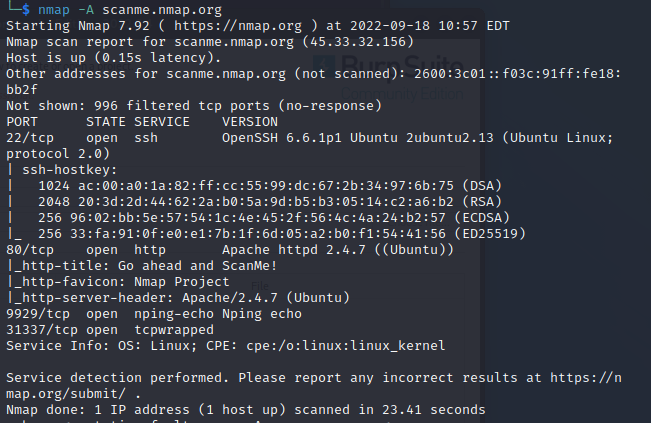
\includegraphics[width=0.5\textwidth]{/home/bruno/git/Praxisbericht_Bacherloarbeit/Praxissemester/assets/nmap.png}
    \caption{Brute force Scan für Verzeichnisentdeckung}
    \centering
\end{figure}

Aus diesem Scan erfahren wir welche Betriebssystem und welche Version der Webanwendung benutzt werden. Auch wenn solche Versionen gegen Angriffe geschützt sind, ist es unsere Aufgabe dem Kunde zu informieren, dass sensitive Informationen für alle sichtbar sind. Eine böse absichtliche Nutzer könnte diese Information nutzen, um eine \glsplural{Schwachstelle} für diese Anwendungen zu erfinden und dann auszunutzen.

\subsection{Ausnutzung der Zielanwendung}

Nachdem die vorherigen Scans durchgeführt wurden und öffentliche Serverseite Informationen gesammelt wurden, fangen wir mit den Tests auf der Webanwendung an. In diesem Fall ist es unser Ziel zu wissen, welche versteckte Daten oder unerlaubte Aktionen ein Angreifer durchführen kann, um die \gls{CIA} der Anwendung zu verletzen. Für die folgenden Tests benutzen wir unter anderen auch das Tool \gls{burp}.

Unser erster Test will überprüfen, ob es möglich ist, in ein Eingabefeld Daten einzutragen und das normale Verhalten der Anwendung zu ändern. Wir wollen eigenen Code hinzuführen und in dem Falle, dass es uns gelingt, das zu tun, können wir dann weitere Code hinzufügen, um Daten von Nutzer zu stehlen oder das normale Verhalten der Anwendung beschädigen. Wir prüfen hier, ob die Anwendung gegen \glsfirst{xss} anfällig ist. Um diesen Test durchzuführen, fügen wir erwartete Daten hinzu, um das Verhalten der Anwendung zu beobachten. Nachdem wir das normale Verhalten erkannt haben, versuchen wir eigenen Code hinzufügen und beobachten, ob wir die Anwendung ausnutzen können. 

\begin{figure}[H]
    \centering
    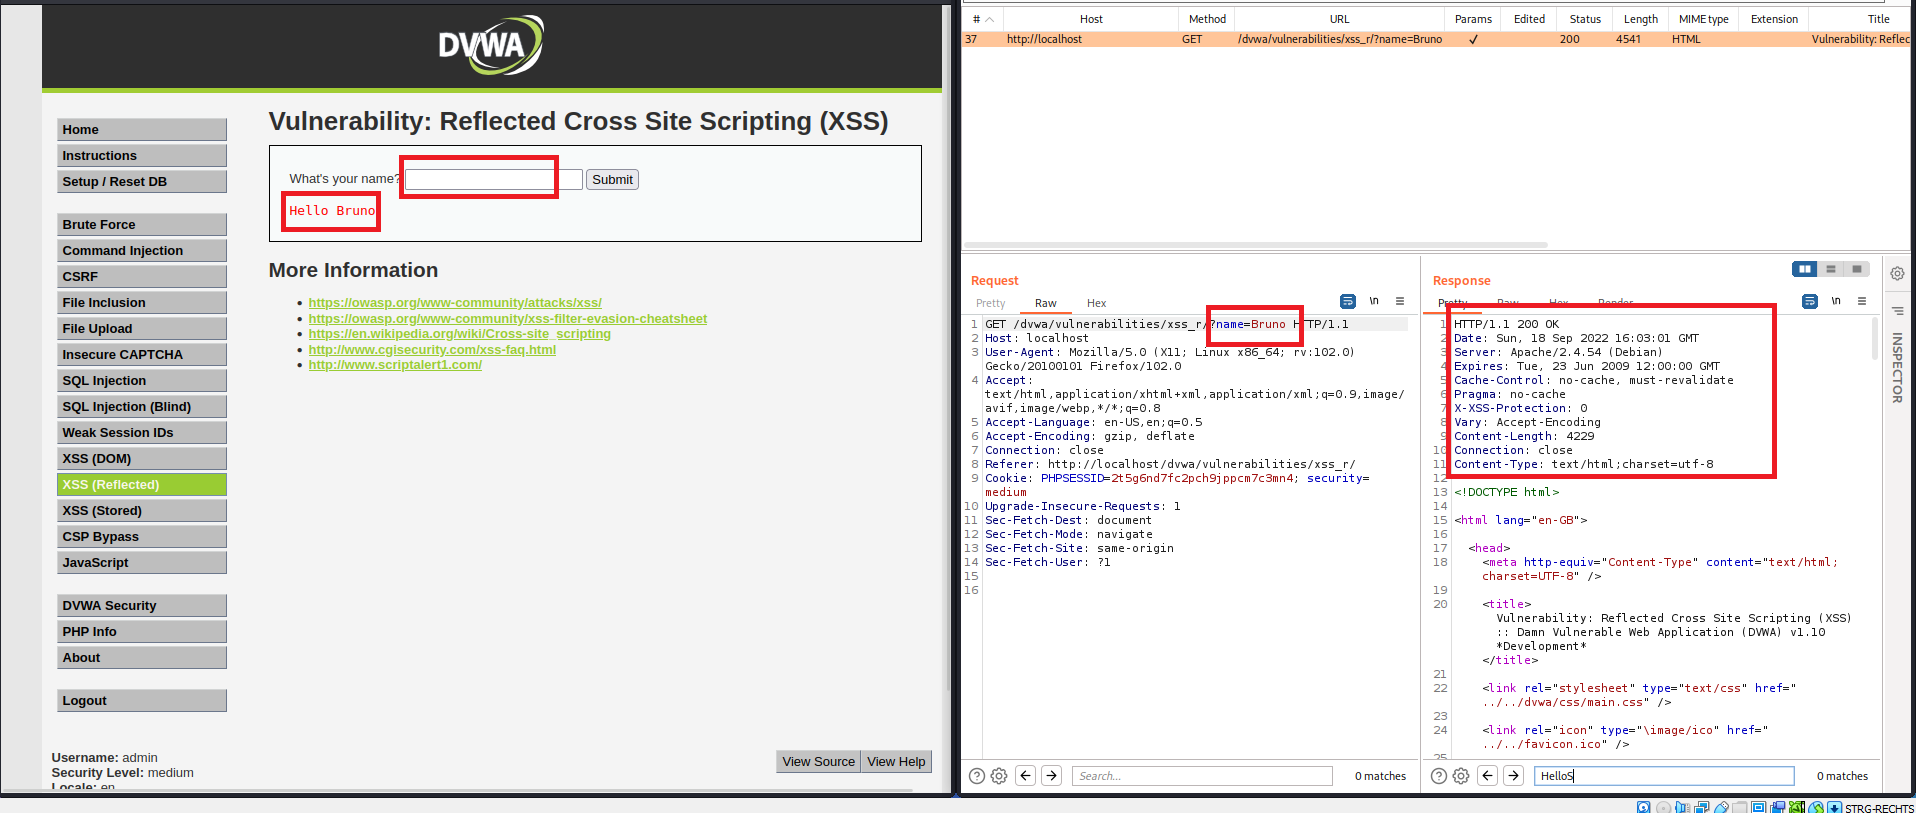
\includegraphics[width=0.8\textwidth]{/home/bruno/git/Praxisbericht_Bacherloarbeit/Praxissemester/assets/xssnormal.png}
    \caption{Beobachtung der Anwendung unter normale Nutzung}
    \label{fig:xssnormal}
    \centering
\end{figure}

Das Bild \ref{fig:xssnormal} zeigt den ersten Test. Aus dieser Aufnahme der Anfrage können wir sehen, sehen, dass die Nutzereingabe direkt in dem Browser stattfindet. Wir sehen in der Antwort Informationen über den Aufbau der Anwendung und wie sie auf unsere Anfrage reagiert. Auf dem nächsten Bild versuchten wir einige bösartige Code hinzufügen, um den normalen Ablauf der Anwendung zu verletzten. Dafür verwenden \gls{javascript} Code. Wir können unseren Code direkt in die Anwendung, in eine selbst gebastelte Request oder in \gls{burp} eingabe:

\begin{figure}[H]
    \centering
    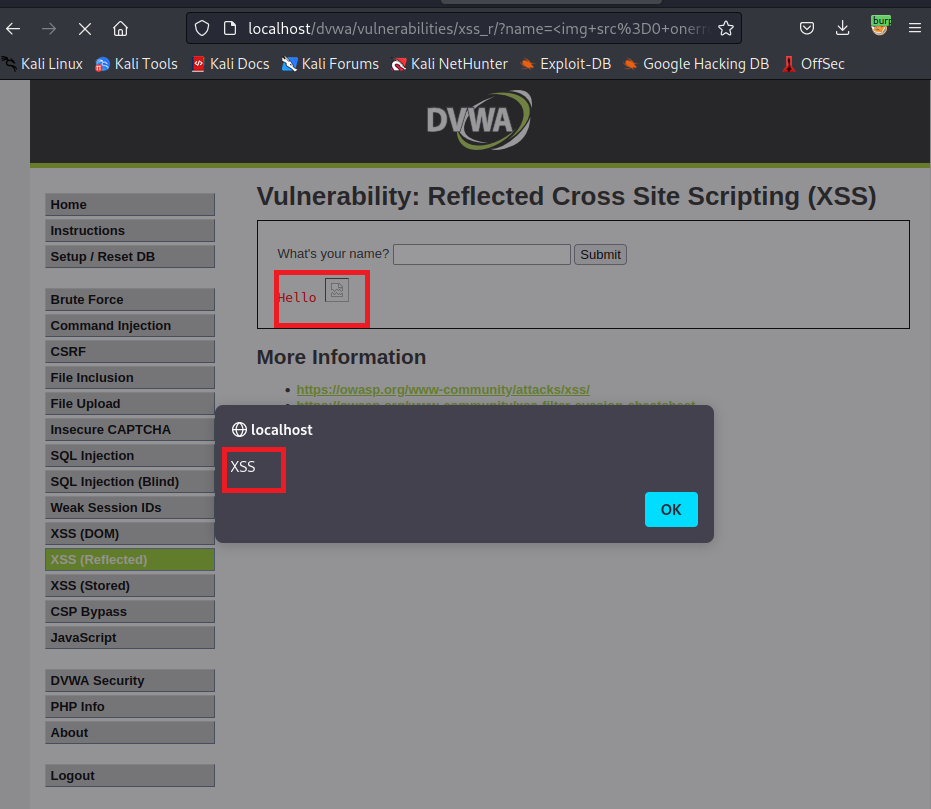
\includegraphics[width=0.8\textwidth]{/home/bruno/git/Praxisbericht_Bacherloarbeit/Praxissemester/assets/xss.png}
    \caption{Einführung von bösartigen Code und Beobachtung der Reaktion der Anwendung.}
    \label{fig:xssexecuted}
    \centering
\end{figure}

Für diesen Test haben wir den Code \textit{<img src=0 onerror='alert(``XXS'')'\textbackslash>} hinzugefügt. Das Ziel dieses Codes ist ein nicht existierende Bild hinzufügen, um einen absichtlichen Fehler zu provozieren. Dieser Fehler zeigt ein kleines Fenster in der Anwendung mit dem Text ```XSS'''. Eine geschützte Anwendung würde entweder den Code und ihren Zeichen ``< >'' ignorieren oder diese zu anderen übersetzen. Es kann auch sein, dass die Anwendung den Nutzer sagt, dass die eingegebenen Zeichen nicht erlaubt nicht. Aus dem Bild sehen wir aber, dass die Anwendung alle Zeichen akzeptiert und sogar erlaubt, dass der Code ausgeführt wird. Aus dieser Situation hätten wir einen \glsfirst{pof}, dass die Anwendung gegen diese Art von Angriff anfällig ist.


\subsection{Kundebericht}

Je nachdem wie lange das Projekt läuft, können wir mehr oder weniger zeitintensive Tests durchführen. Am Ende des Projekts präsentieren wir dem Beauftragten in einem Meeting unser Ergebnis und liefern wir ein Bericht mit detaillierte Informationen über die gefundenen \glsplural{Schwachstelle} und die dazu verwendete Methode, um sie zu finden. Dieses Bericht wird so geschrieben, damit non-native Nutzer es verstehen können. 

In den ersten Abschnitten erklären wir mit weniger technischen Begriffe, wie was für Tests durchgeführt wurden. In den folgenden Kapitel erklären wir mit mehr Einzelheiten und technische Details, wie wir zu unserem Ergebnis kamen. Anschließend geben wir Vorschläge für die Verbesserung der Sicherheit der Webanwendung und am Ende geben wir mithilfe von \gls{CVSS} oder von den Kunden ausgewählten Metrik eine allgemeine Bewertung.
